\documentclass{standalone}
\usepackage[all]{xy}
\usepackage{bm}
\usepackage{tikz}

\usetikzlibrary{shapes.arrows, shapes.geometric}
\tikzstyle{line} = [thick,->]
\tikzstyle{arrow} = [
	thick,
	->,
	>=stealth,
	black,
]
\tikzstyle{agente} = [
	rectangle, 
	minimum width=1cm, 
	minimum height=1cm,
	text centered,
	draw=black, 
	fill=green!30
]
\tikzstyle{modelo} = [
	rectangle, 
	rounded corners,
	minimum width=1cm, 
	minimum height=1cm,
	text centered,
	draw=black, 
	fill=red!30
]
\tikzstyle{memoria} = [
	rectangle, 
	rounded corners,
	minimum width=1cm, 
	minimum height=1cm,
	text centered,
	draw=black, 
	fill=gray!30
]
\tikzstyle{entorno} = [
	rectangle, 
	minimum width=1cm, 
	minimum height=1cm,
	text centered, 
	draw=black, 
	fill=blue!15
]


\begin{document}

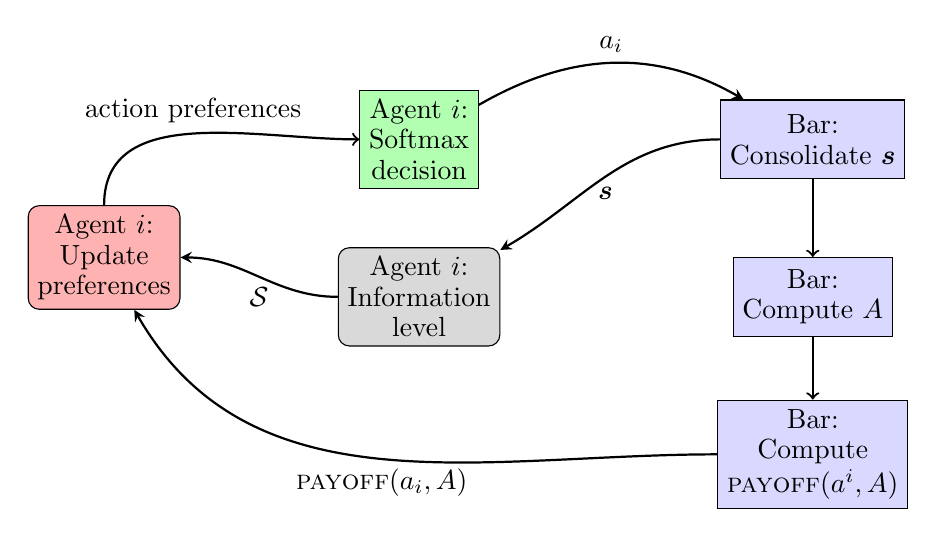
\begin{tikzpicture}
\node[agente] (A) at (0,2) {\txt{Agent $i$:\\Softmax\\ decision}};
\node[entorno] (B) at (5,2) {\txt{Bar:\\Consolidate $\bm{s}$}};
\node[entorno] (C) at (5,0) {\txt{Bar:\\Compute $A$}};
\node[entorno] (D) at (5,-2) {\txt{Bar:\\Compute\\ $\textsc{payoff}(a^i, A)$}};
\node[memoria] (E) at (0,0) {\txt{Agent $i$:\\Information\\level}};
\node[modelo] (F) at (-4,0.5) {\txt{Agent $i$:\\Update\\preferences}};
\draw[arrow] (A) edge [out=30, in=150, anchor=south] node {$a_i$} (B);
%\draw[arrow] (A) edge [anchor=east] node {$a_i$} (E);
\draw[line] (B) -- (C);
\draw[line] (C) -- (D);
\draw[arrow] (B) edge [out=180, in=30, anchor=north] node {$\bm{s}$} (E);
\draw[arrow] (D) edge [out=180, in=-60, anchor=north] node {$\textsc{payoff}(a_i, A)$} (F);
\draw[line] (F) edge [out=90, in=180, anchor=south] node {action preferences} (A);
\draw[arrow] (E) edge [out=180, in=0, anchor=north] node {$\mathcal{S}$} (F);
\end{tikzpicture}

\end{document}